\section{CRM: oportunidades y embudo de ventas}

El CRM (Gestión de Relaciones con Clientes) es el corazón de tus ventas. Aquí es donde registras a toda persona que pregunta por un tour, le haces seguimiento y finalmente logras que te compren.

% ─────────────────────────────────────────────────────────────────────────────
\subsection{Abrir el CRM y ver tu embudo}

Cuando entras al CRM, verás una pantalla muy visual con columnas. Esto se llama tu ``Embudo de ventas''.

\begin{figure}[H]
    \centering
    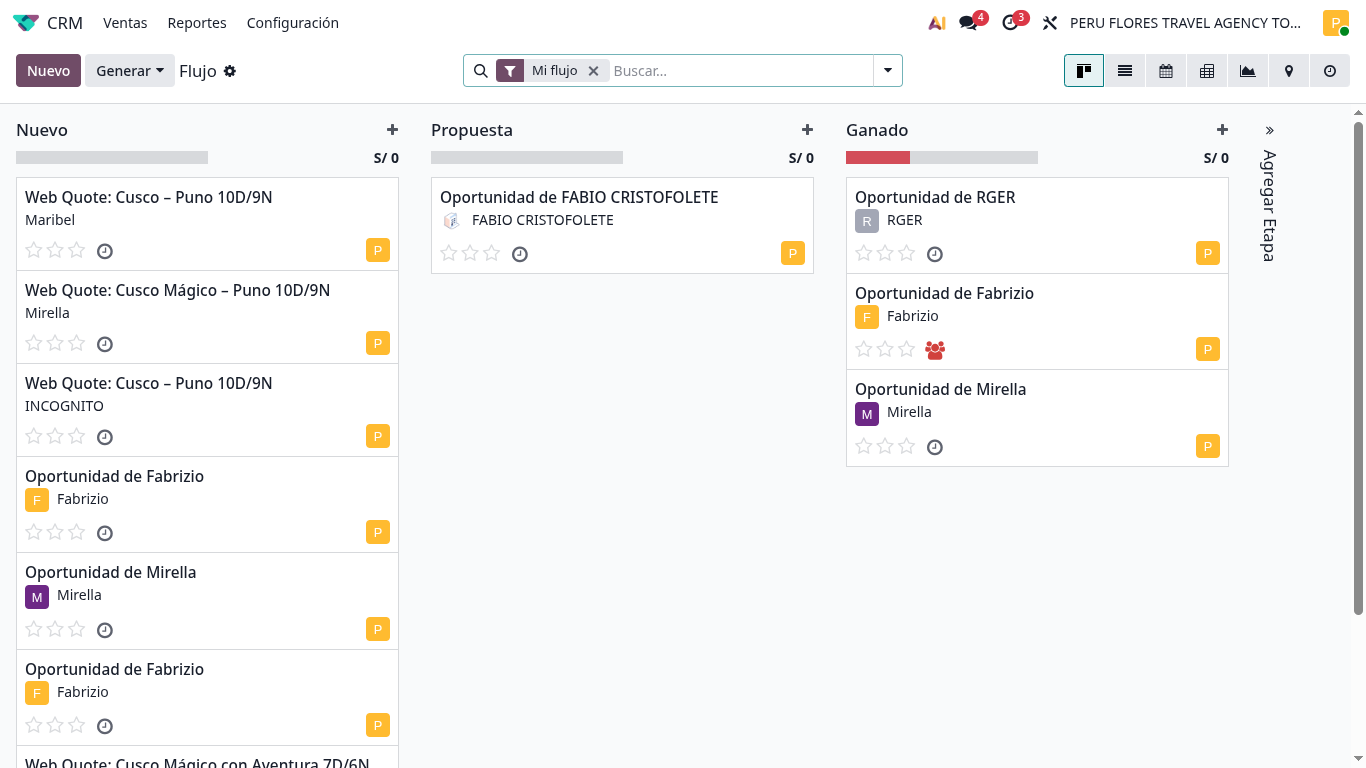
\includegraphics[width=0.9\textwidth]{assets/crm_01_kanban.png}
    \caption{El embudo de ventas. Cada tarjeta es un cliente interesado, y cada columna es un paso en la venta.}
\end{figure}

Sigue estos pasos:
\begin{enumerate}
    \item En la pantalla principal de Odoo, haz clic en la aplicación \textbf{``CRM''}.
    \item Verás varias columnas como ``Nuevo'', ``Calificado'', ``Propuesta'' y ``Ganado''.
    \item Cada tarjetita blanca que ves ahí es una \textbf{Oportunidad} de venta (alguien que preguntó por un tour).
\end{enumerate}

% ─────────────────────────────────────────────────────────────────────────────
\subsection{Crear una oportunidad nueva}

Cada vez que te escriba un pasajero nuevo por WhatsApp o correo pidiendo información, debes crear una tarjetita para él de inmediato.

\begin{figure}[H]
    \centering
    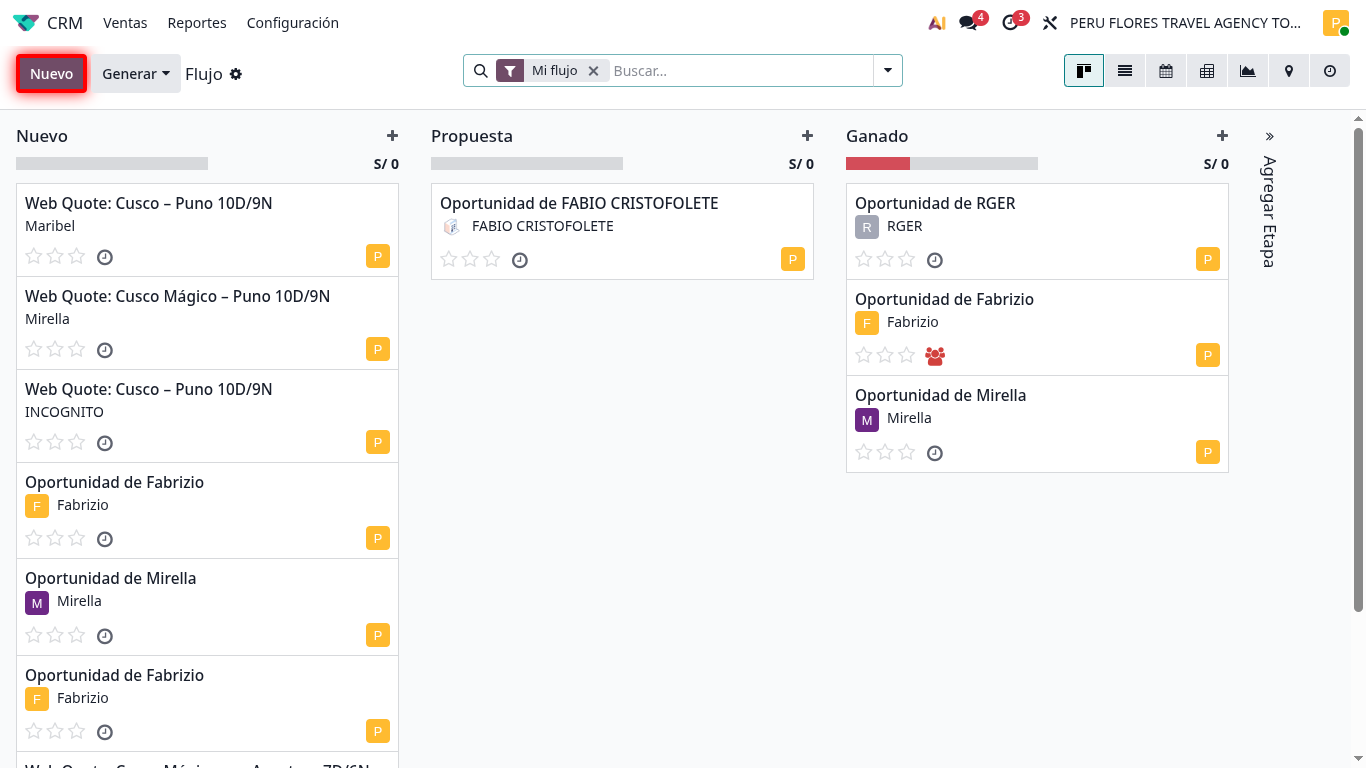
\includegraphics[width=0.9\textwidth]{assets/crm_02_nuevo_highlight.png}
    \caption{El botón \textbf{``Nuevo''} (marcado en rojo) en la parte superior izquierda.}
\end{figure}

Sigue estos pasos:
\begin{enumerate}
    \item En la esquina superior izquierda, haz clic en el botón que dice \textbf{``Nuevo''} (marcado en rojo en la imagen superior).
    \item Aparecerá una pequeña tarjetita en blanco en la primera columna para que llenes los datos básicos rápidamente.
\end{enumerate}

\begin{figure}[H]
    \centering
    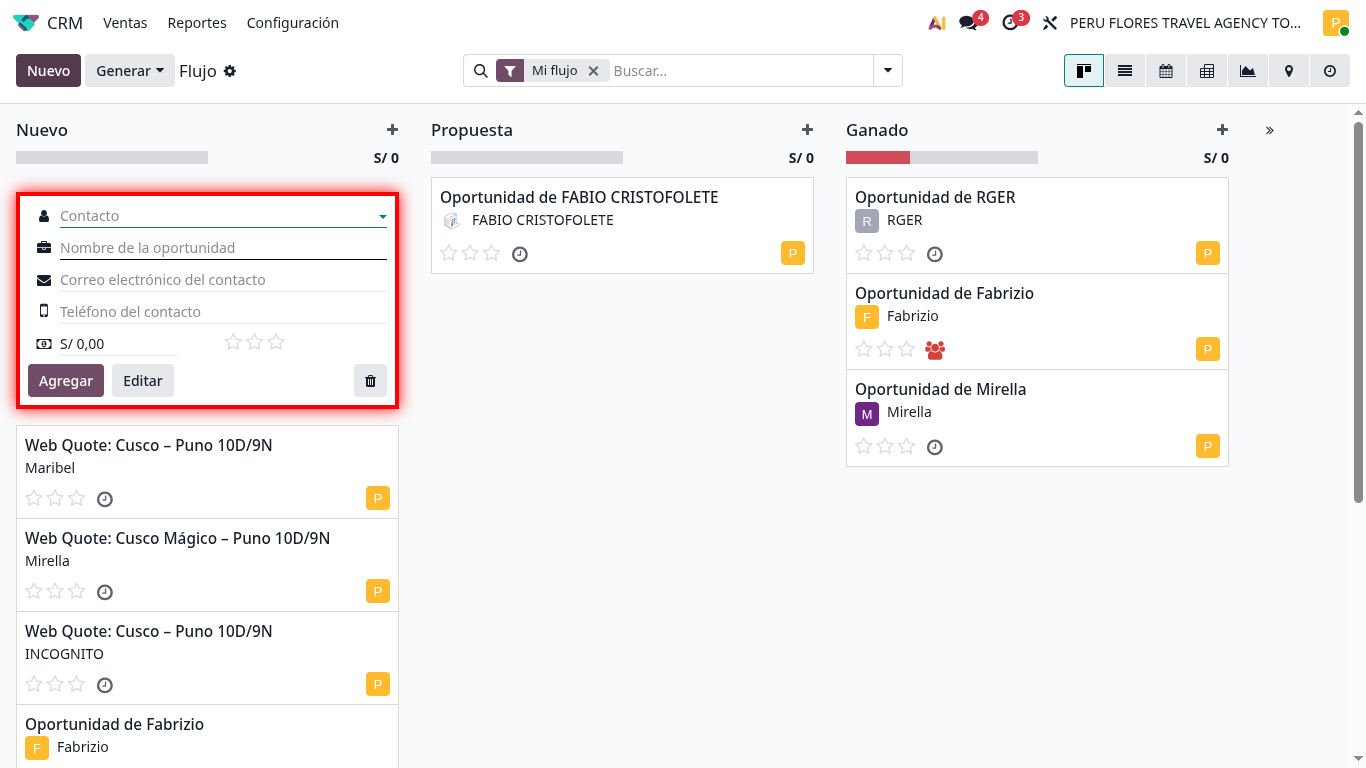
\includegraphics[width=0.6\textwidth]{assets/crm_10_quick_create_box.png}
    \caption{La ventanita rápida para registrar la oportunidad, con sus campos básicos.}
\end{figure}

\begin{enumerate}
    \setcounter{enumi}{2}
    \item Escribe un título para la oportunidad (ejemplo: ``Tour Machu Picchu 2 PAX'').
    \item En el campo de cliente, escribe el nombre del pasajero.
    \item En el campo de ingreso esperado, pon un aproximado de cuánto dinero crees que costará el tour.
    \item Haz clic en el botón oscuro que dice \textbf{``Añadir''} para guardar la tarjeta en el embudo, o en \textbf{``Editar''} si quieres abrir la ficha completa al instante.
\end{enumerate}

% ─────────────────────────────────────────────────────────────────────────────
\subsection{Completar la información de la oportunidad}

Una vez creada la oportunidad, debes abrirla para llenarla con todos los detalles importantes.

\begin{figure}[H]
    \centering
    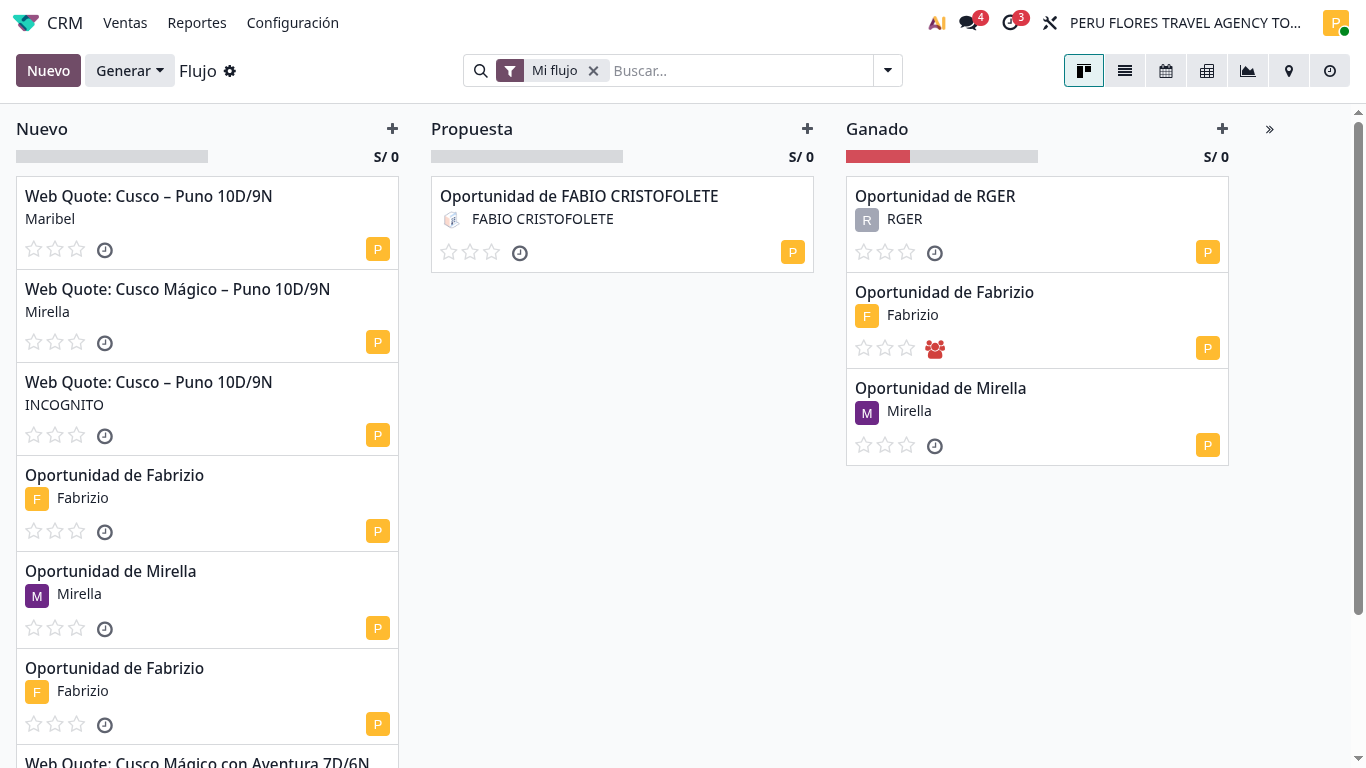
\includegraphics[width=0.9\textwidth]{assets/crm_04_form_completo.png}
    \caption{La ficha completa de la oportunidad donde pones todos los detalles de la venta.}
\end{figure}

\begin{figure}[H]
    \centering
    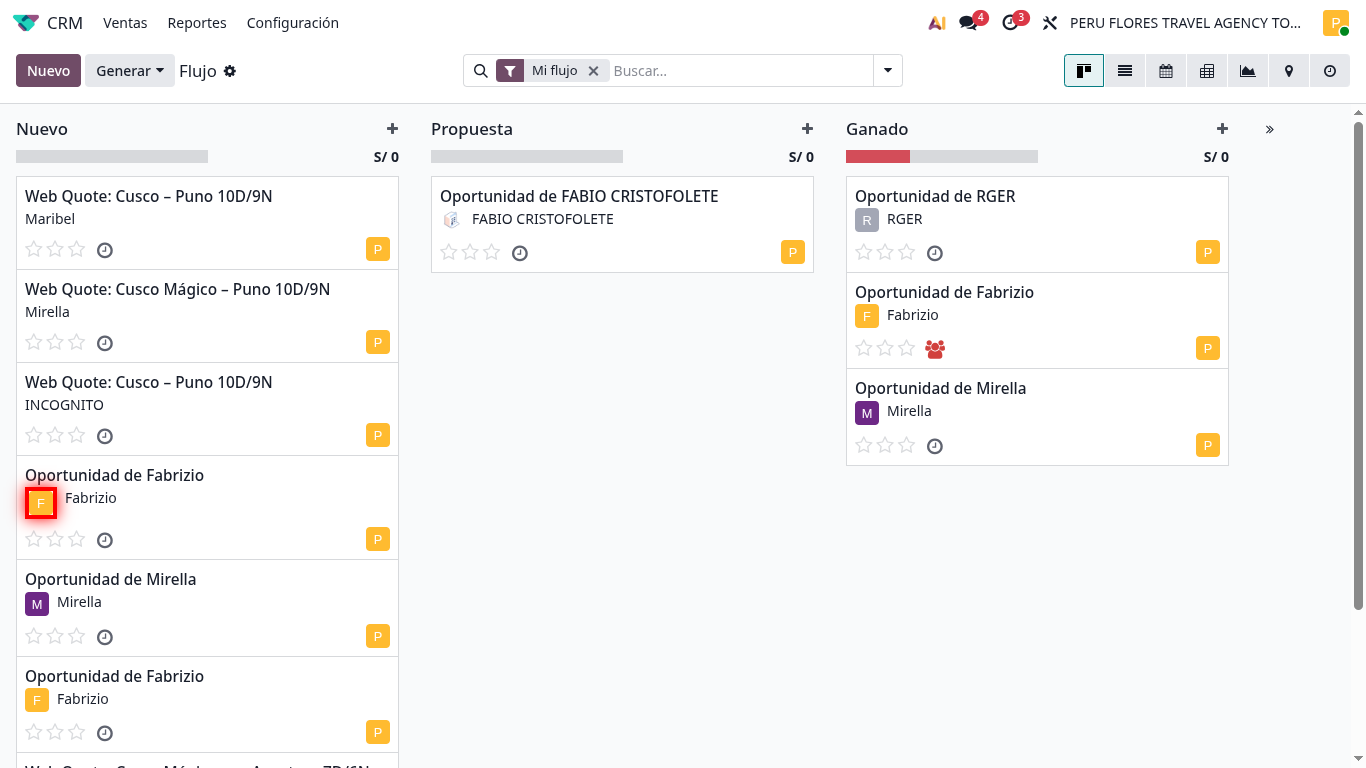
\includegraphics[width=0.9\textwidth]{assets/crm_08_cliente_highlight.png}
    \caption{El campo de \textbf{Cliente} (marcado en rojo). Si el cliente no existe, puedes crearlo directamente desde aquí.}
\end{figure}

Sigue estos pasos:
\begin{enumerate}
    \item Haz clic sobre la tarjeta de la oportunidad en el embudo para abrirla.
    \item Asegúrate de vincularla a un cliente. En el campo marcado en rojo en la segunda imagen, escribe el nombre del cliente. Si no lo habías guardado en tus contactos antes, el sistema te dará la opción de \textbf{``Crear''} uno nuevo al instante.
    \item Escribe fechas estimadas, correos y usa la zona de abajo (el Chatter) para dejar notas internas (ejemplo: ``El pasajero viaja con un niño'').
\end{enumerate}

% ─────────────────────────────────────────────────────────────────────────────
\subsection{Mover la oportunidad en el embudo}

Para que tengas orden, la tarjeta debe moverse de columna en columna a medida que avanzas en la conversación con el cliente.

Sigue estos pasos:
\begin{enumerate}
    \item Ve a la pantalla principal del CRM (el embudo).
    \item Haz clic izquierdo sobre la tarjeta del cliente y \textbf{mantenlo presionado}.
    \item Arrastra la tarjeta hacia la derecha, a la columna que corresponda (por ejemplo, si ya le enviaste los precios, muévela a la columna ``Propuesta'').
    \item Suelta el clic. Así sabrás siempre en qué estado está cada venta.
\end{enumerate}

% ─────────────────────────────────────────────────────────────────────────────
\subsection{Todo lo que puedes hacer dentro de la ficha de oportunidad}

Una vez que abres la ficha completa de un cliente interesado (la ``cartilla''), tienes varias herramientas poderosas para cerrar la venta.

\begin{figure}[H]
    \centering
    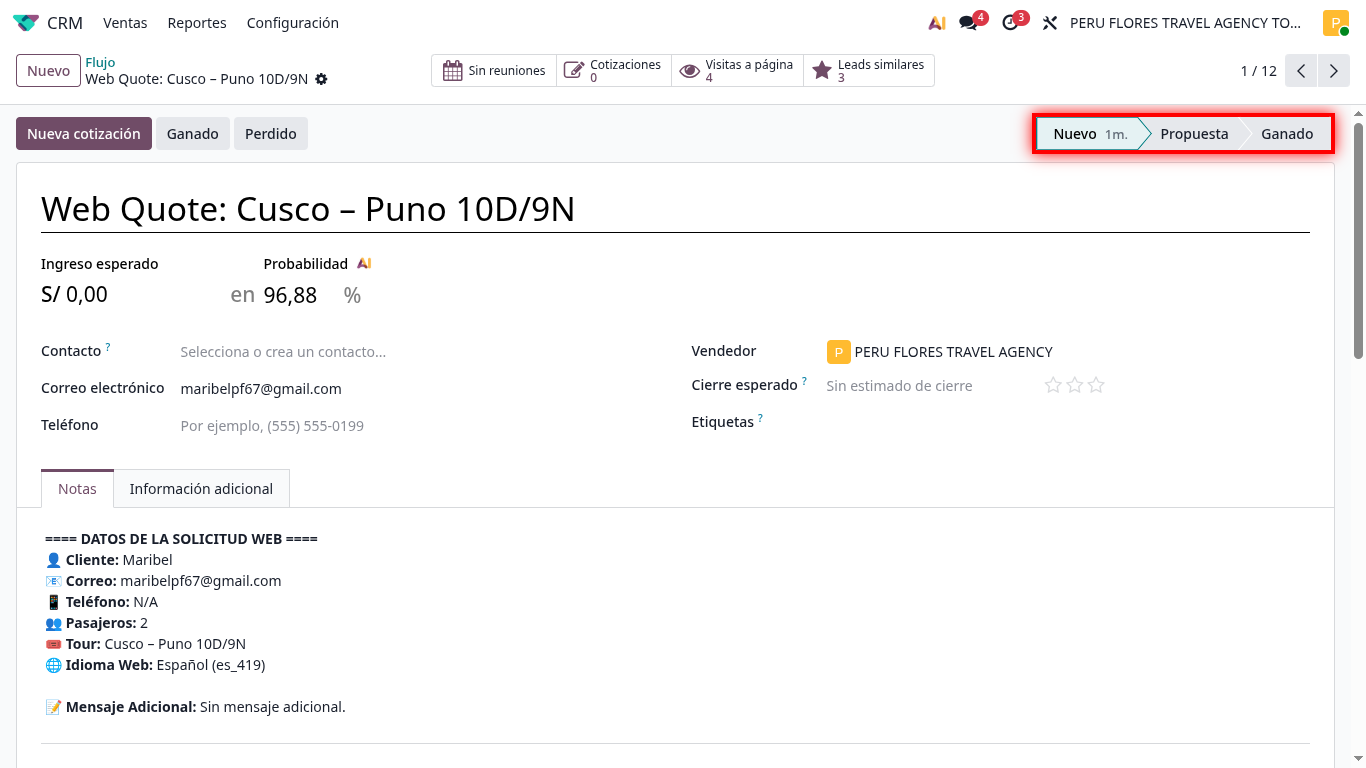
\includegraphics[width=0.9\textwidth]{assets/crm_15_detalle_etapas.png}
    \caption{La barra superior que muestra en qué etapa se encuentra la venta (marcada en rojo).}
\end{figure}

\textbf{1. Cambiar la etapa sin salir de la ficha:} 
No necesitas arrastrar la tarjeta en el embudo si ya estás adentro. Simplemente haz clic en las palabras de la barra superior (ej. ``Propuesta'') para avanzar la venta.

\begin{figure}[H]
    \centering
    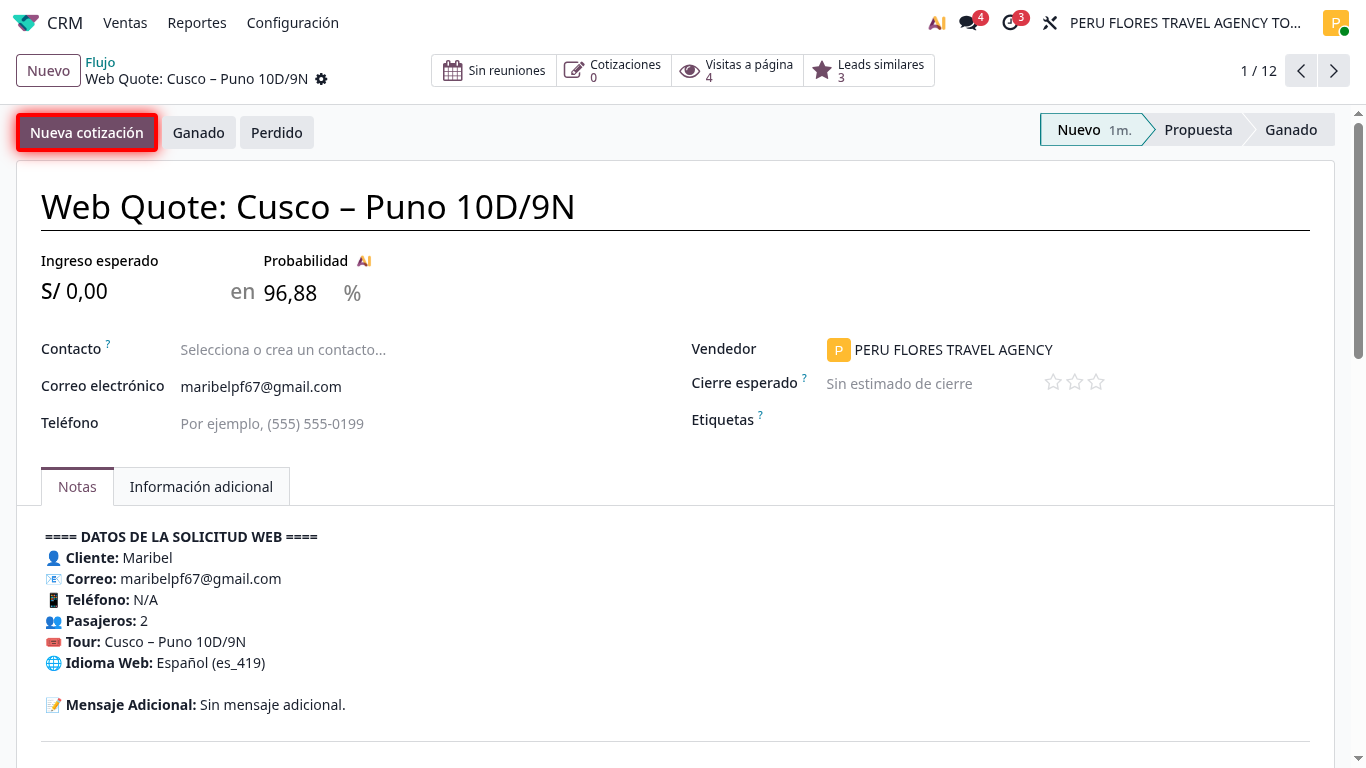
\includegraphics[width=0.9\textwidth]{assets/crm_16_detalle_nueva_cotizacion.png}
    \caption{El botón \textbf{``Nueva cotización''} (marcado en rojo) para enviarle los precios al cliente.}
\end{figure}

\textbf{2. Generar una cotización oficial:} 
Si el cliente ya te pidió precios formales, haz clic en el botón \textbf{``Nueva cotización''}. Esto te abrirá un documento de venta con los datos del pasajero ya precargados, listo para que agregues los tours y se lo envíes por correo.

\begin{figure}[H]
    \centering
    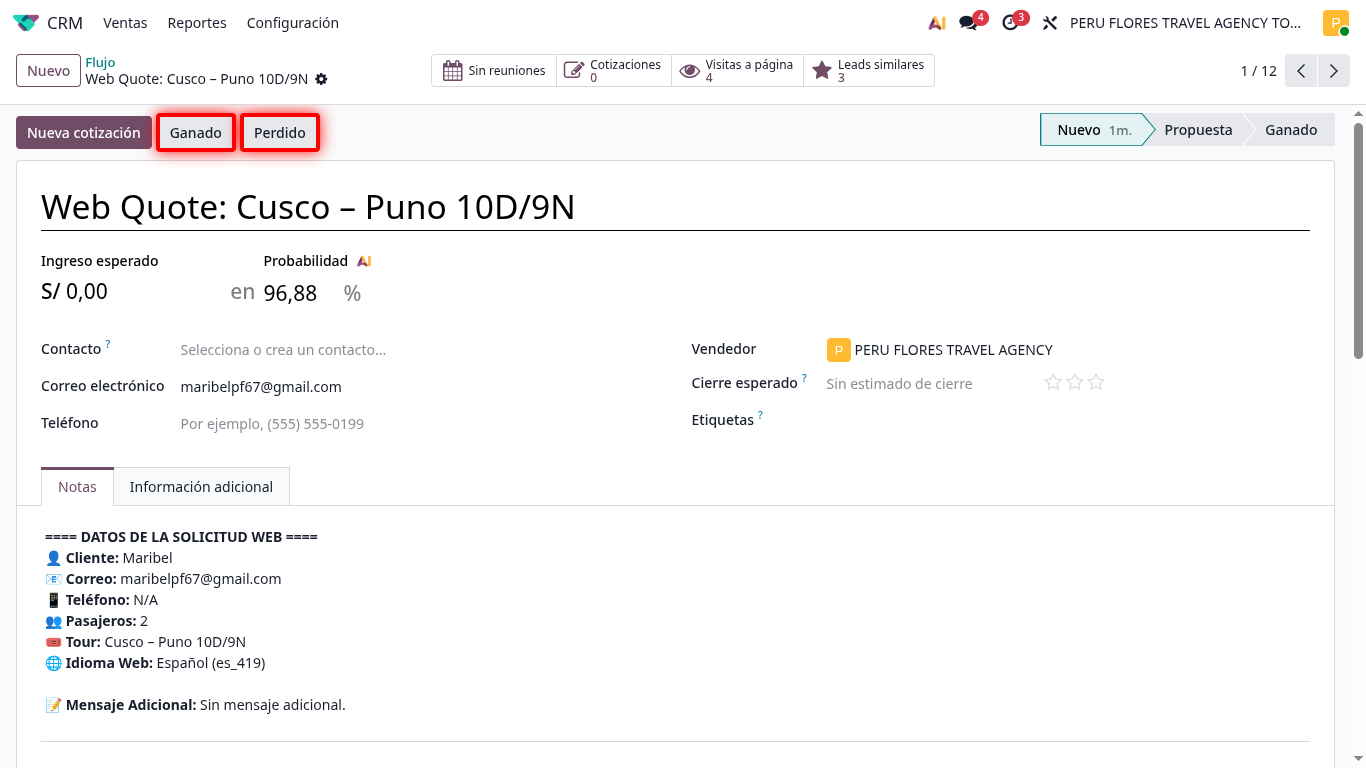
\includegraphics[width=0.9\textwidth]{assets/crm_17_detalle_ganado_perdido.png}
    \caption{Los botones de \textbf{``Ganado''} y \textbf{``Perdido''} para cerrar el caso.}
\end{figure}

\textbf{3. Cerrar la venta (Ganado / Perdido):} 
El objetivo final del CRM es vender. 
\begin{itemize}
    \item Si el cliente acepta el precio y te paga o confirma, haz clic en el botón verde \textbf{``Ganado''}. ¡La tarjeta se pintará con una franja verde, celebrando tu éxito!
    \item Si el cliente ya no viajará o te dice que compró en otra agencia, haz clic en el botón \textbf{``Perdido''}. El sistema te preguntará el motivo (ej. ``Muy caro'') para que en el futuro sepas por qué pierdes ventas, y la tarjeta desaparecerá del embudo para no estorbarte.
\end{itemize}

\textbf{4. Usar el registro interno (Chatter):} 
Debajo de los datos del cliente verás una zona donde puedes hacer clic en \textbf{``Registrar nota''}. Úsalo como un cuaderno de apuntes (ej. ``Llamé al cliente pero no contestó, volver a intentar mañana''). También puedes usar \textbf{``Planificar actividad''} para que el sistema te recuerde llamarlo o enviarle un correo en una fecha específica.
